\documentclass[11pt,a4paper]{article}

\usepackage[utf8]{inputenc}
\usepackage[T1]{fontenc}
\usepackage[spanish,es-noshorthands]{babel}
\usepackage[margin=2.3cm]{geometry}
\usepackage{graphicx}
\usepackage{xcolor}
\usepackage{booktabs}
\usepackage{tabularx}
\usepackage{array}
\usepackage{longtable}
\usepackage{enumitem}
\usepackage{listings}
\usepackage{fancyhdr}
\usepackage{titlesec}
\usepackage[hidelinks]{hyperref}
\usepackage{caption}

\definecolor{ink}{HTML}{1F2937}
\definecolor{accent}{HTML}{6C3483}
\definecolor{codebg}{HTML}{0F172A}
\definecolor{codefg}{HTML}{E2E8F0}
\definecolor{crit}{HTML}{C0392B}
\definecolor{high}{HTML}{E67E22}
\definecolor{med}{HTML}{D4AC0D}
\definecolor{low}{HTML}{27AE60}
\definecolor{rowg}{HTML}{F4F6F7}

\hypersetup{colorlinks=true,linkcolor=accent,urlcolor=accent}

\titleformat{\section}{\Large\bfseries\color{ink}}{\thesection.}{0.5em}{}
\titleformat{\subsection}{\large\bfseries\color{ink}}{\thesubsection}{0.5em}{}
\titlespacing*{\section}{0pt}{16pt}{6pt}

\pagestyle{fancy}\fancyhf{}
\lhead{\small\color{ink}FinSight --- Informe Final DevSecOps}
\rhead{\small\color{ink}UTEC}
\cfoot{\small\thepage}
\renewcommand{\headrulewidth}{0.4pt}

\newcolumntype{Y}{>{\raggedright\arraybackslash}X}
\newcommand{\sev}[1]{\textbf{\textcolor{#1}}}

\lstdefinestyle{yaml}{
  basicstyle=\ttfamily\scriptsize\color{codefg},
  backgroundcolor=\color{codebg},
  breaklines=true, breakatwhitespace=false,
  frame=single, framerule=0pt, rulecolor=\color{codebg},
  xleftmargin=6pt, xrightmargin=6pt, aboveskip=8pt, belowskip=8pt,
  showstringspaces=false, keepspaces=true, columns=fullflexible,
}

\setlist{topsep=2pt,itemsep=1pt}

\begin{document}

% ---------------- Portada ----------------
\begin{center}
  {\LARGE\bfseries\color{ink} Presentación Final del Proyecto}\\[4pt]
  {\large\bfseries Informe Final --- DevSecOps}\\[14pt]
  {\Huge\bfseries\color{accent} FinSight}\\[6pt]
  {\normalsize Gestor de finanzas personales \emph{privacy-first} para LATAM con auto-categorización por IA}\\[10pt]
  \href{https://github.com/bylenz/finsight}{\texttt{https://github.com/bylenz/finsight}}\\[14pt]
\end{center}

\noindent\textbf{Curso:} DevOps --- UTEC \quad\textbullet\quad \textbf{Semana 16} \quad\textbullet\quad \textbf{Valor:} 30\% de la nota final

\vspace{6pt}
\begin{center}
\begin{tabularx}{\linewidth}{@{}l Y@{}}
\toprule
\textbf{Rol} & \textbf{Integrante} \\
\midrule
Tech Lead / DevOps & Lenin Chávez \\
Backend \& Security Lead & Jerimy Sandoval \\
AI \& Analytics Lead & Adrian Céspedes \\
Frontend Dev & Lenin Chávez, Adrian Céspedes \\
QA / Test Strategy & Jerimy Sandoval \\
\bottomrule
\end{tabularx}
\end{center}

\vspace{4pt}
\hrule
\vspace{10pt}

% ---------------- 1. Objetivo ----------------
\section{Objetivo}
Exponer de forma sintética y clara los resultados obtenidos a lo largo del proyecto integrador
FinSight, destacando la aplicación práctica de los conceptos de \textbf{DevOps} y \textbf{DevSecOps}:
modelado de amenazas STRIDE, integración de análisis de seguridad (SAST, DAST, secret scanning y
SCA) en el pipeline de CI/CD, centralización de hallazgos en DefectDojo, y las lecciones aprendidas
y recomendaciones para futuras implementaciones en entornos de desarrollo ágil y continuo.

% ---------------- a. Título y descripción ----------------
\section{Título y descripción del proyecto}
\textbf{FinSight} es un \emph{personal finance tracker} basado en web con IA conversacional en español,
construido para el mercado latinoamericano. Los usuarios registran gastos por voz, texto o CSV; la IA
los categoriza automáticamente, detecta patrones de gasto y emite alertas de presupuesto. La aplicación
es \emph{privacy-first} (no requiere credenciales bancarias) y soporta multi-moneda (PEN, USD) y hogares
multi-usuario.

\vspace{4pt}
\noindent\textbf{Arquitectura (resumen):}
\begin{itemize}
  \item \textbf{Frontend:} Streamlit (\texttt{frontend/src/finsight\_ui}).
  \item \textbf{Backend:} FastAPI (\texttt{backend/src/finsight}) --- módulos \texttt{auth}, \texttt{expenses},
        \texttt{budgets}, \texttt{categories}, \texttt{households}, \texttt{dashboard}, \texttt{exports}, \texttt{insights}.
  \item \textbf{Base de datos:} PostgreSQL 16 (SQLAlchemy async + Alembic).
  \item \textbf{Autenticación:} JWT (python-jose) + bcrypt (12 rounds).
  \item \textbf{Servicio externo:} Anthropic LLM para categorización de gastos.
  \item \textbf{Infraestructura:} Docker Compose; CI/CD en GitHub Actions.
\end{itemize}

% ---------------- b. Diagrama STRIDE ----------------
\section{Diagrama de modelado de amenazas (STRIDE)}
Diagrama de flujo de datos con fronteras de confianza (\emph{trust boundaries}). Cada arista se anota con
las categorías STRIDE aplicables. Versión editable en draw.io: \texttt{docs/informe-final/stride-finsight.drawio}.

\begin{center}
  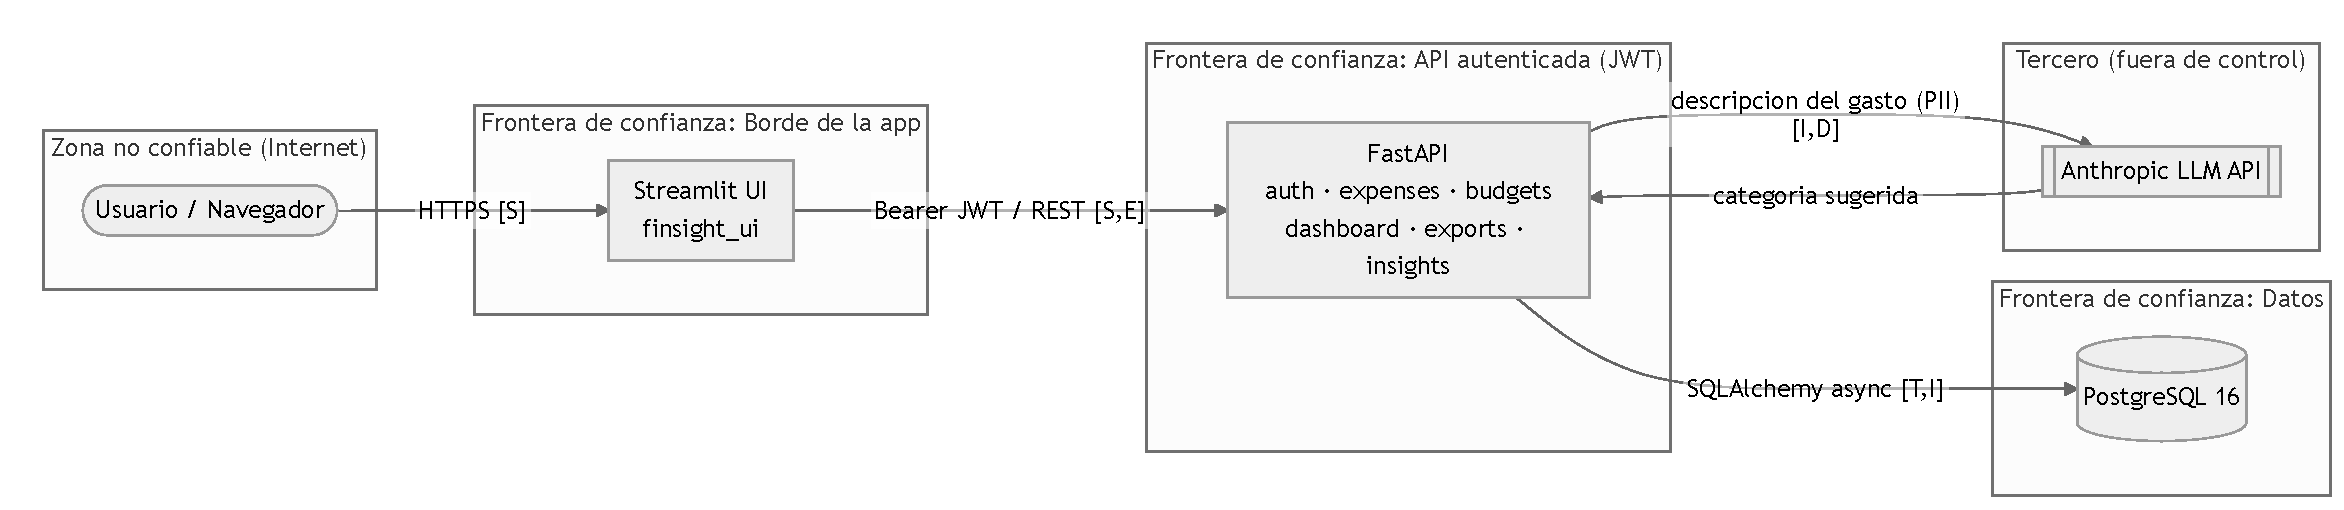
\includegraphics[width=\linewidth]{images/stride.pdf}
\end{center}

\noindent\footnotesize S=Spoofing \textbullet\ T=Tampering \textbullet\ R=Repudiation \textbullet\
I=Information Disclosure \textbullet\ D=Denial of Service \textbullet\ E=Elevation of Privilege
\normalsize

% ---------------- c. 5 vulnerabilidades ----------------
\section{Cinco vulnerabilidades principales (STRIDE)}
\renewcommand{\arraystretch}{1.25}
\begin{tabularx}{\linewidth}{@{}l l Y@{}}
\toprule
\textbf{Threat Type} & \textbf{Componente} & \textbf{Descripción de la amenaza} \\
\midrule
\textcolor{crit}{\textbf{Spoofing}} & Login / JWT &
Reuso de un JWT robado o falsificado para suplantar a un usuario. El token incluía \texttt{jti} pero
\textbf{no existía lista de revocación} y vivía 24h; la seguridad dependía además del \texttt{SECRET\_KEY}. \\
\textcolor{crit}{\textbf{Tampering}} & expenses / budgets &
\textbf{Broken Object-Level Authorization (IDOR):} un miembro podía leer o modificar recursos de otro
hogar alterando el \texttt{id} en la petición si faltaban chequeos de pertenencia. \\
\textcolor{high}{\textbf{Info. Disclosure}} & insights (LLM) / exports &
Las \textbf{descripciones de gastos (PII)} se envían a un tercero (Anthropic) para categorizar; ese dato
sale del perímetro. Una exportación CSV mal autorizada podría filtrar gastos de otro hogar. \\
\textcolor{high}{\textbf{Denial of Service}} & FastAPI / LLM &
\textbf{Sin rate limiting:} un atacante satura la API o abusa de la categorización por IA (cada gasto
nuevo dispara una llamada al LLM), generando \emph{cost-based DoS}. \\
\textcolor{high}{\textbf{Elev. of Privilege}} & households / dependencias &
Un rol \texttt{viewer} ejecutando acciones de \texttt{owner}; o una \textbf{dependencia vulnerable}
(p.\,ej. CVE en \texttt{python-jose}) con ruta a ejecución de código y escalamiento. \\
\bottomrule
\end{tabularx}

\vspace{4pt}
\noindent\emph{Repudiation (brecha identificada):} no existía \emph{audit logging} de eventos de seguridad,
por lo que las acciones no eran trazables ni atribuibles.

% ---------------- d. SAST y DAST ----------------
\section{Elección de herramientas SAST y DAST}
\textbf{SAST (análisis estático):} \textbf{Semgrep} (reglas \texttt{p/ci}, \texttt{p/security-audit},
\texttt{p/python}) + \textbf{Bandit} (analizador específico de Python).\\
\textbf{DAST (análisis dinámico):} \textbf{OWASP ZAP} \emph{baseline scan} contra el contenedor del backend
levantado en CI.

\vspace{3pt}
\noindent\textbf{Evidencia de integración:} las tres herramientas corren como \emph{jobs} del workflow
\texttt{.github/workflows/security.yml} (GitHub Actions) --- ver §11. Cada una exporta un reporte JSON
(\texttt{semgrep-report.json}, \texttt{bandit-report.json}, \texttt{zap-report.json}) que se publica como
artefacto de CI y se centraliza en DefectDojo (§8). Ejecución local reproducible: Semgrep y Bandit generaron
hallazgos de severidad baja sobre \texttt{backend/src/finsight}, visibles en el dashboard de la §8.

% ---------------- e. Secret scanning y SCA ----------------
\section{Elección de herramientas de Secret Scanning y SCA}
\textbf{Secret Scanning:} \textbf{Gitleaks} + \textbf{TruffleHog} (\texttt{--results=verified,unknown}), más
el hook \texttt{detect-private-key} de \emph{pre-commit} como primera barrera local.\\
\textbf{SCA (dependencias):} \textbf{Trivy} (\texttt{filesystem} sobre las dependencias + escaneo de la
imagen Docker) y generación de \textbf{SBOM} en formato CycloneDX.

\vspace{3pt}
\noindent\textbf{Doble barrera:} \emph{pre-commit} bloquea secretos localmente y el pipeline vuelve a
validarlos en CI. \textbf{Evidencia:} en la ejecución real Gitleaks reportó \emph{sin fugas}; TruffleHog,
Trivy y el SBOM produjeron sus reportes (\texttt{gitleaks-report.json}, \texttt{trufflehog-report.json},
\texttt{trivy-fs-report.json}, \texttt{sbom.json}) e ingresaron a DefectDojo.

% ---------------- f. DefectDojo ----------------
\section{Centralización de vulnerabilidades en DefectDojo}
Se desplegó \textbf{DefectDojo} localmente con Docker Compose (puerto \texttt{:8082}) y se centralizaron
todos los hallazgos de los escáneres en un único dashboard de deuda técnica de seguridad. Jerarquía:
Product Type \texttt{Aplicaciones Web} $\rightarrow$ Product \texttt{FinSight} $\rightarrow$ Engagement
\texttt{CI Security Scan} $\rightarrow$ un Test por herramienta. La ingesta usa el endpoint
\texttt{POST /api/v2/reimport-scan/} (deduplicación con \texttt{close\_old\_findings}) mediante el script
\texttt{scripts/upload\_to\_defectdojo.sh}.

\vspace{4pt}
\begin{center}
  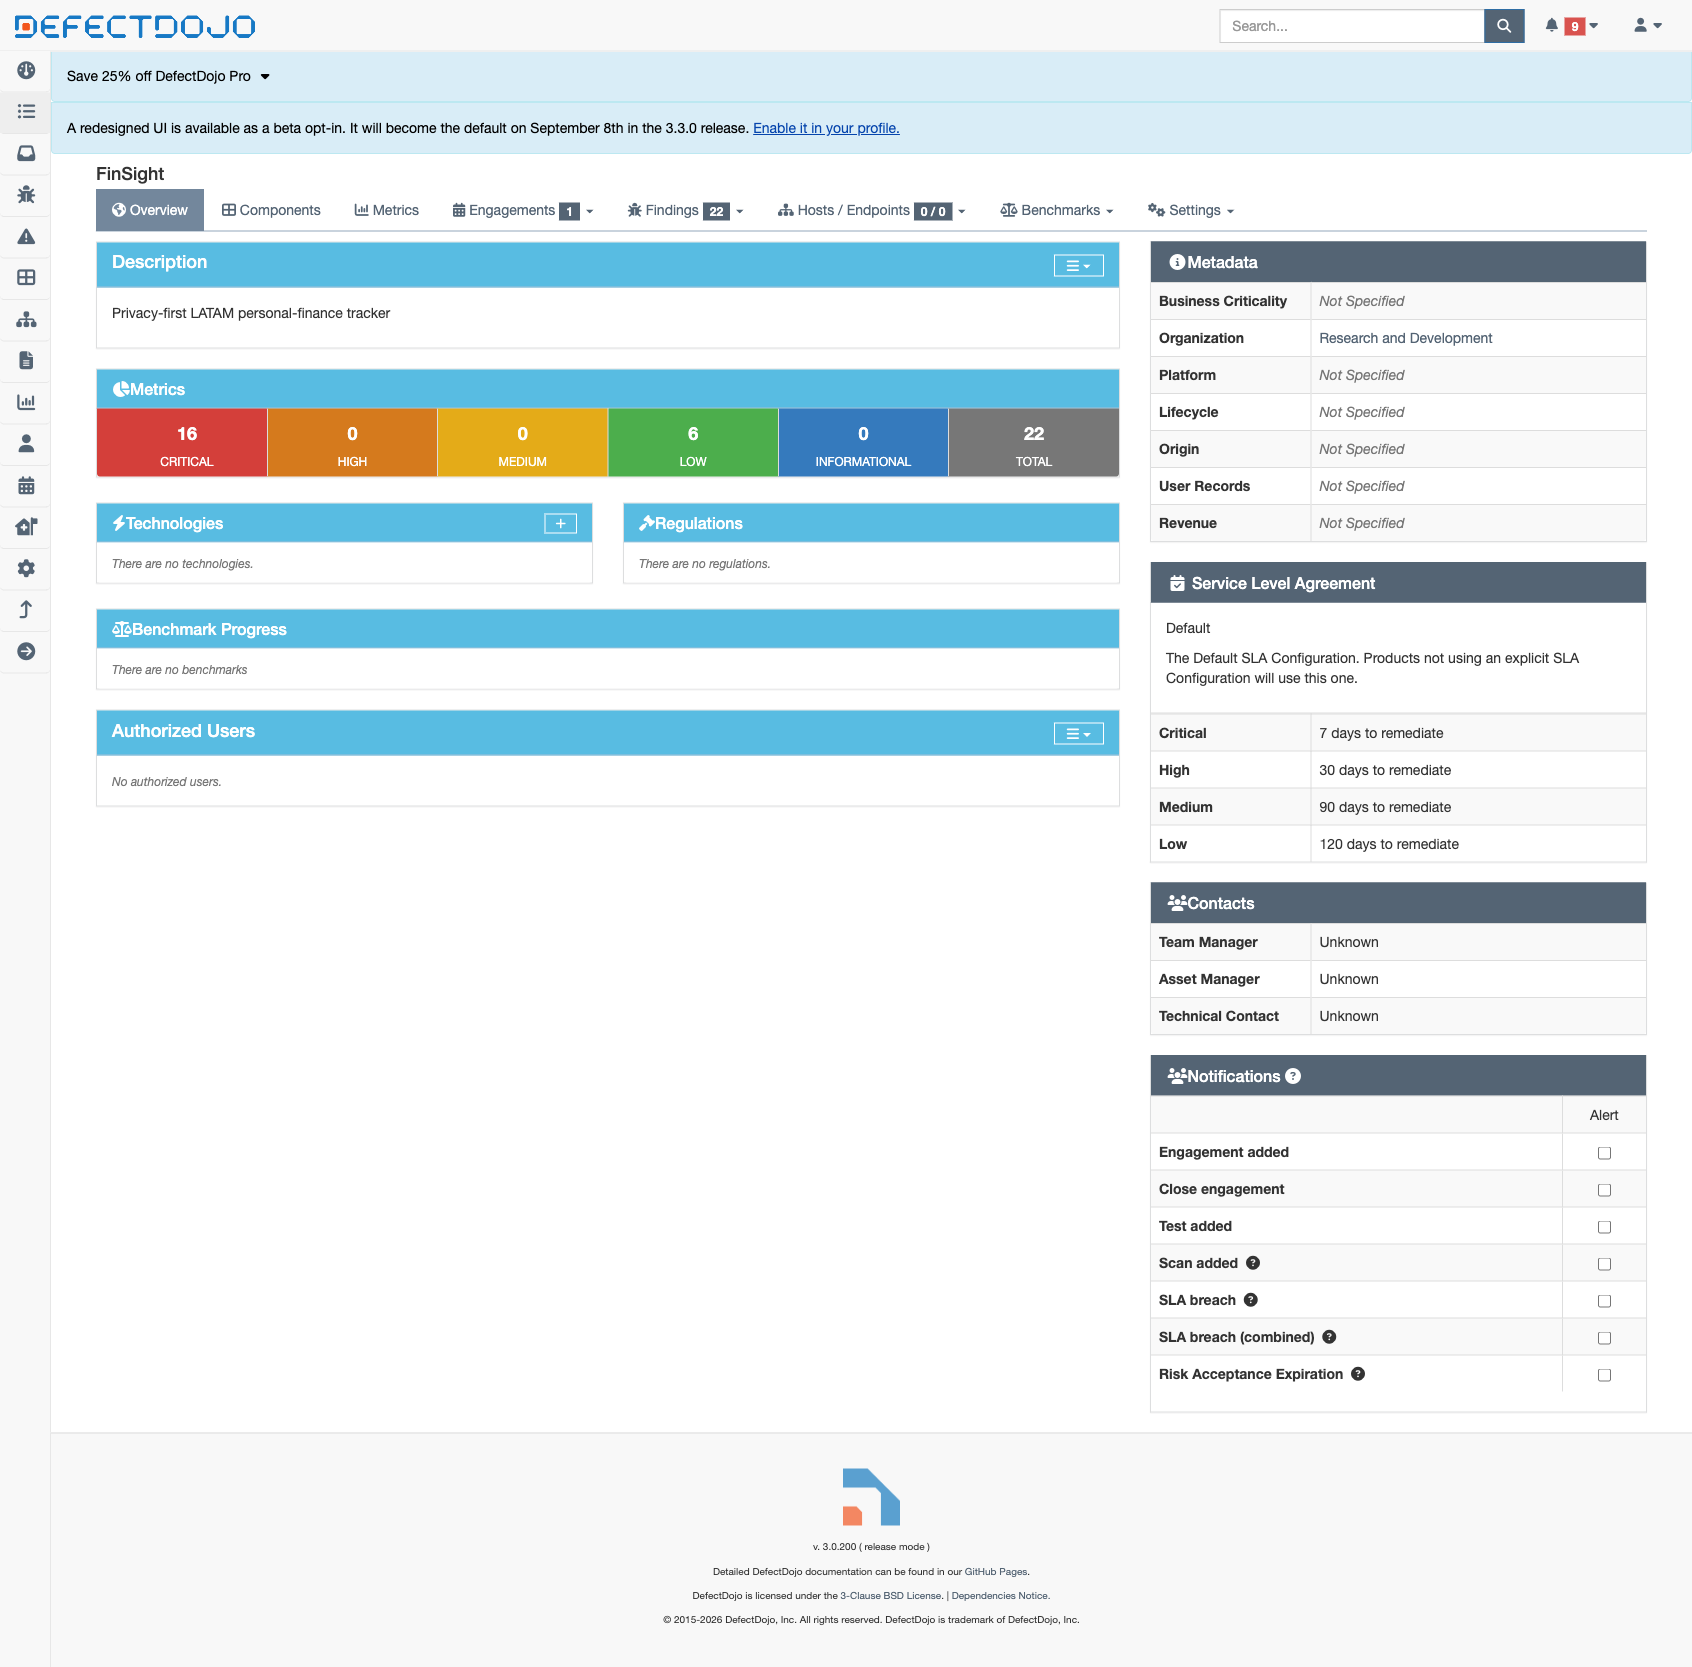
\includegraphics[width=\linewidth]{images/dd-product-finsight.png}
  \captionof{figure}{DefectDojo --- Product \texttt{FinSight}: 22 hallazgos por severidad y 5 escaneos (Gitleaks, TruffleHog, Trivy, Semgrep, Bandit).}
\end{center}

\begin{center}
  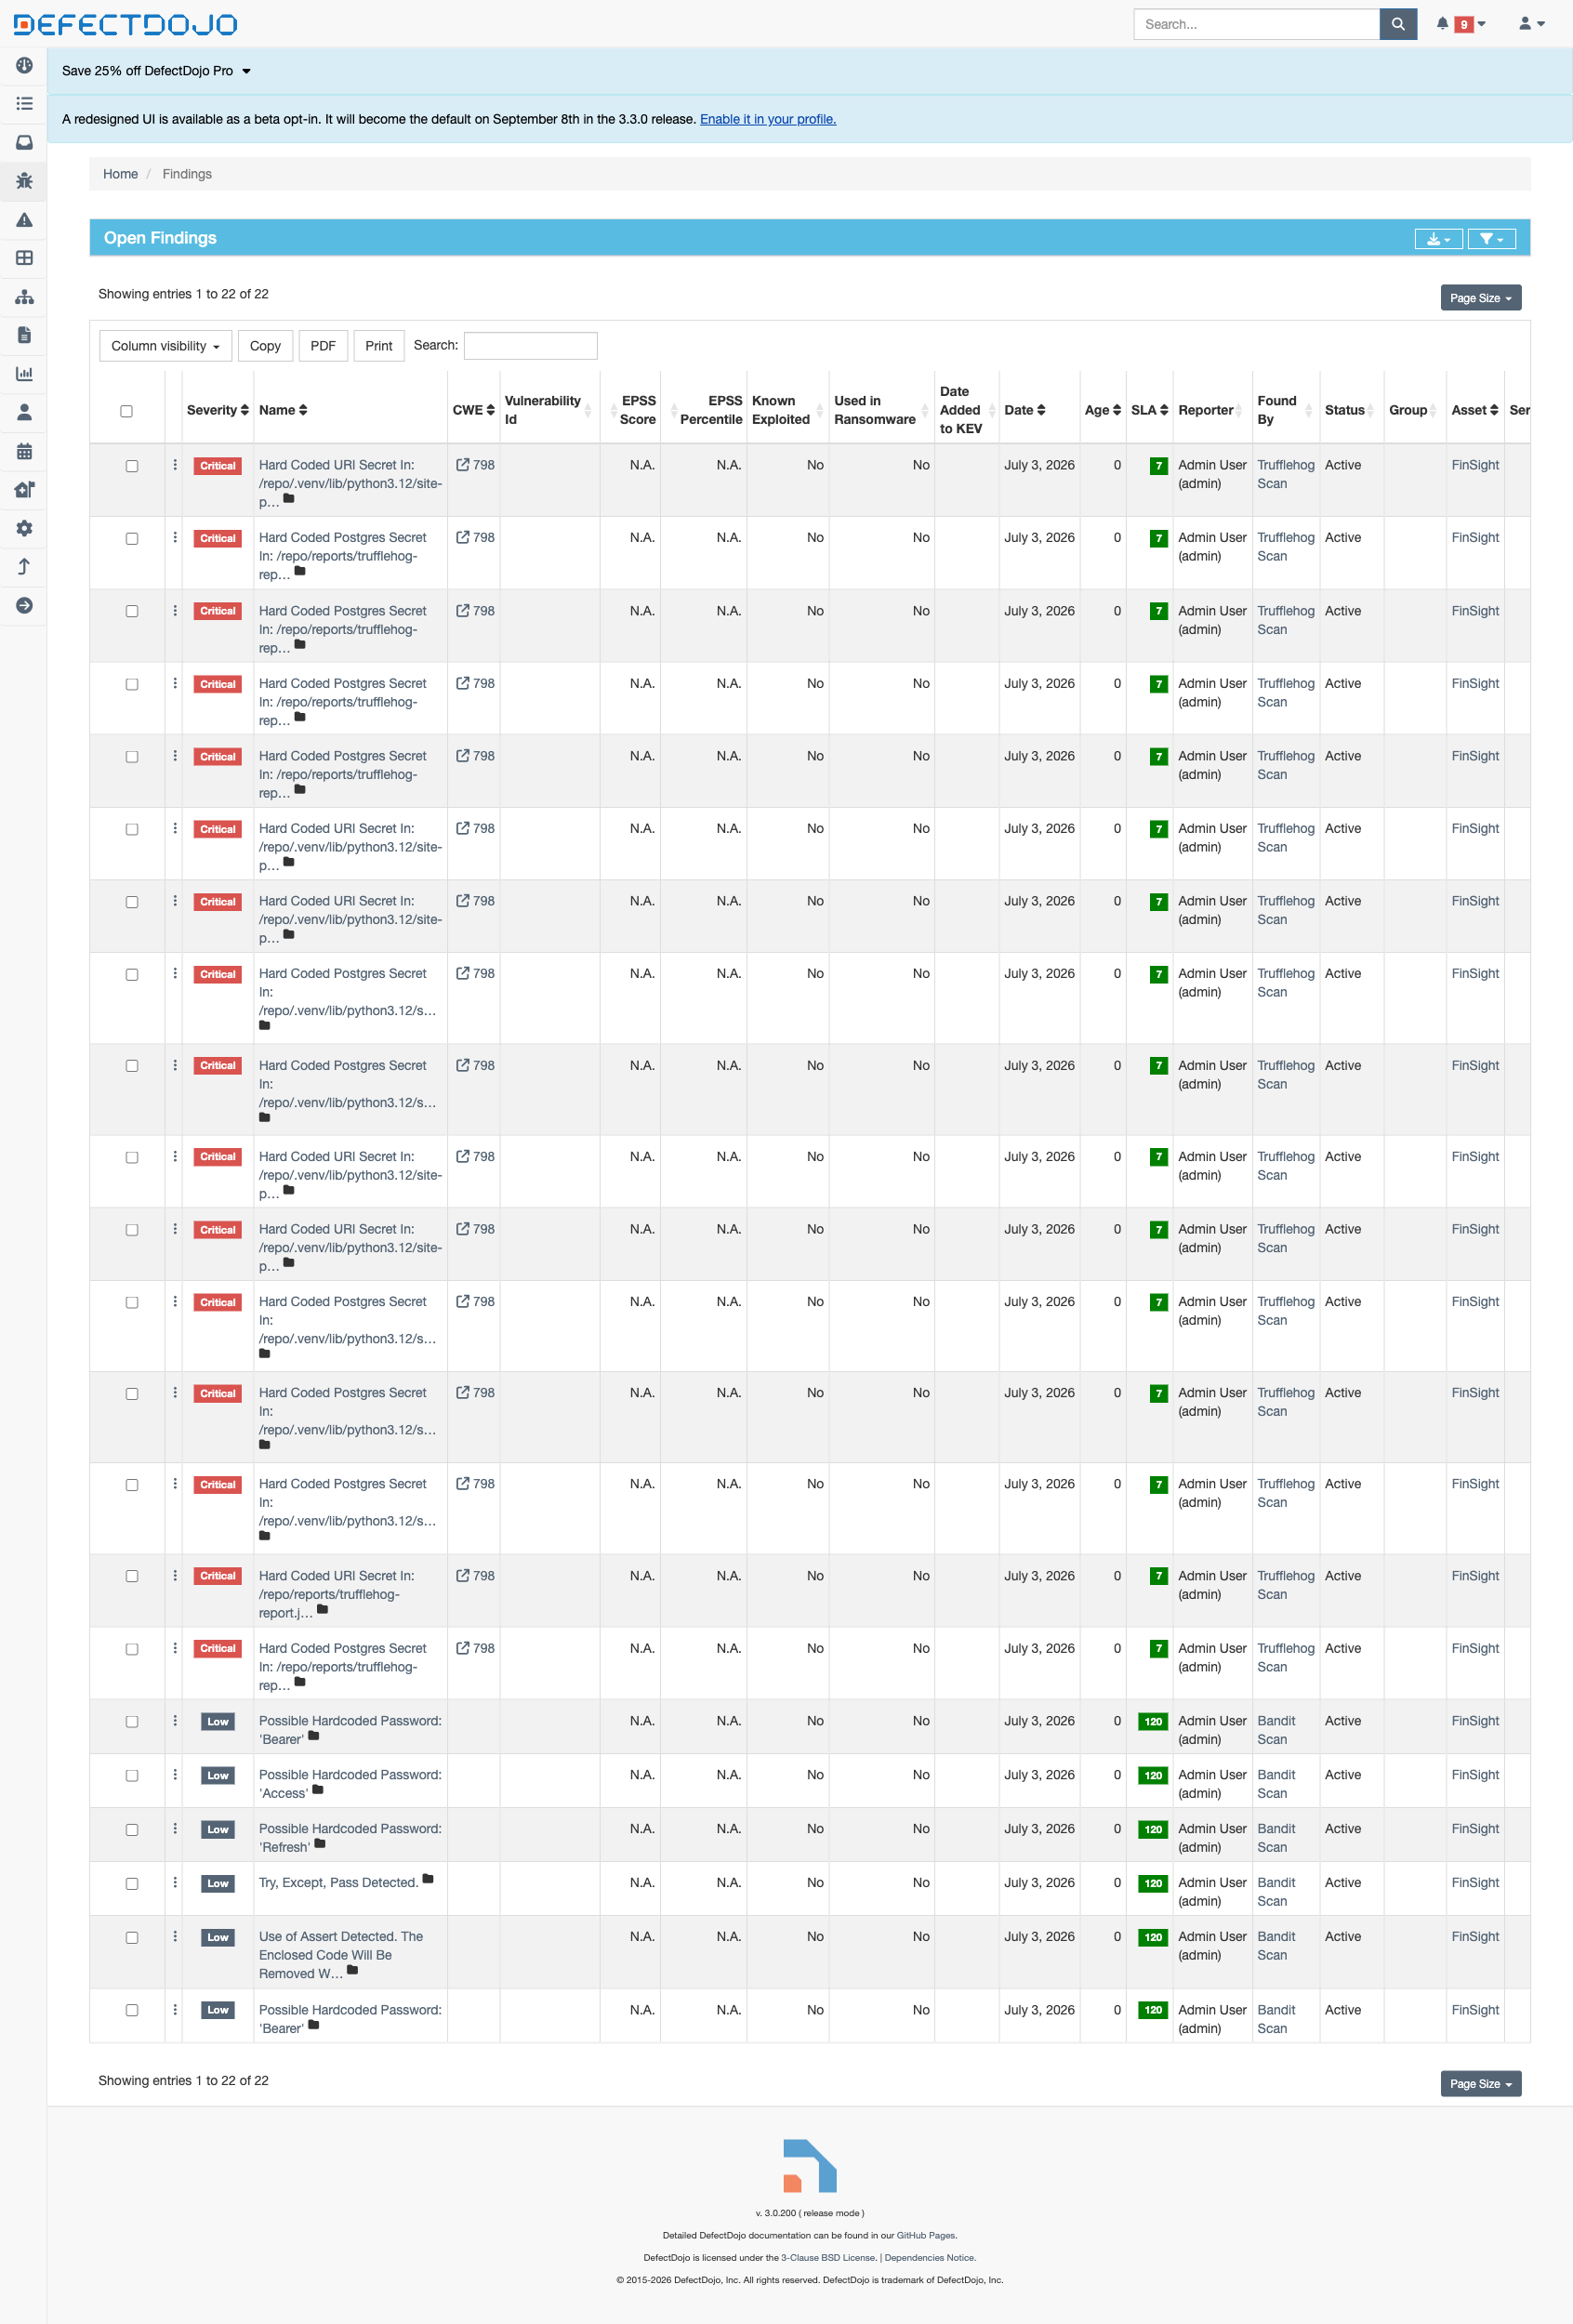
\includegraphics[width=\linewidth]{images/dd-findings-open.png}
  \captionof{figure}{DefectDojo --- listado de hallazgos abiertos centralizados.}
\end{center}

\noindent\footnotesize Nota: los 16 hallazgos \emph{Critical} son candidatos de TruffleHog
(\texttt{--results=verified,unknown}), en su mayoría sin verificar (tokens de ejemplo / fixtures de test),
no secretos reales en producción.\normalsize

% ---------------- g. Tabla de mitigaciones ----------------
\section{Tabla de mitigaciones (hallazgos priorizados)}
\renewcommand{\arraystretch}{1.3}
\begin{tabularx}{\linewidth}{@{}l Y l l Y@{}}
\toprule
\textbf{ID} & \textbf{Descripción del hallazgo} & \textbf{Sev.} & \textbf{Herramienta} & \textbf{Recomendación / estado} \\
\midrule
CRIT-001 & Posible CVE en dependencia transitiva con ruta a ejecución de código & \textcolor{crit}{CRITICAL} & Trivy / pip-audit & Actualizar a versión segura; fijar en el lock. \emph{Detectado por pipeline.} \\
HIGH-001 & IDOR en \texttt{expenses}/\texttt{budgets} entre hogares & \textcolor{high}{HIGH} & Semgrep / revisión & Validar \texttt{household\_id}/\texttt{user\_id}. \emph{Mitigado (PR \#21).} \\
HIGH-002 & JWT sin revocación; token filtrado válido 24h & \textcolor{high}{HIGH} & STRIDE & Denylist por \texttt{jti} + refresh + TTL 15\,min. \emph{Mitigado (PR \#23).} \\
MED-001 & PII enviada al LLM sin minimización & \textcolor{med}{MEDIUM} & STRIDE / DAST & Minimizar/anonimizar; opt-in. \emph{Parcial (PR \#22).} \\
MED-002 & API sin rate limiting $\rightarrow$ DoS / abuso de costo LLM & \textcolor{med}{MEDIUM} & OWASP ZAP & SlowAPI + circuit breaker. \emph{Mitigado (PR \#22).} \\
LOW-001 & Sin secret scanning en CI previo & \textcolor{low}{LOW} & Gitleaks / TruffleHog & Integrar en pre-commit y pipeline. \emph{Mitigado (PR \#19).} \\
\bottomrule
\end{tabularx}

% ---------------- h. Situación inicial y resultados ----------------
\section{Situación inicial vs. resultados}
\renewcommand{\arraystretch}{1.25}
\begin{tabularx}{\linewidth}{@{}Y c Y@{}}
\toprule
\textbf{Métrica} & \textbf{Antes} & \textbf{Después} \\
\midrule
Herramientas de seguridad en CI & 0 & 5 (Gitleaks, TruffleHog, Trivy+SBOM, Semgrep, Bandit) + ZAP (DAST) \\
Hallazgos visibles / centralizados & 0 (invisibles) & 22 en DefectDojo (16 Critical, 6 Low) \\
Gestión de vulnerabilidades & Ninguna & Dashboard DefectDojo por severidad/herramienta \\
Barreras contra secretos & 1 (detect-private-key) & 3 (detect-private-key + Gitleaks + TruffleHog) \\
Vulnerabilidades STRIDE mitigadas en código & 0 & 4 (IDOR, rate-limit, refresh tokens, audit log) \\
\bottomrule
\end{tabularx}

\vspace{4pt}
\noindent\textbf{Situación inicial:} el CI sólo ejecutaba \texttt{lint} + \texttt{test}; las vulnerabilidades
eran \emph{invisibles}. \textbf{Resultados:} pipeline con etapas de seguridad, hallazgos centralizados y
priorizados en DefectDojo, doble barrera de secretos, y 4 amenazas STRIDE mitigadas en el código.

% ---------------- i. Pipeline ----------------
\section{Pipeline CI/CD completo}
\subsection{Diagrama del pipeline}
\begin{center}
  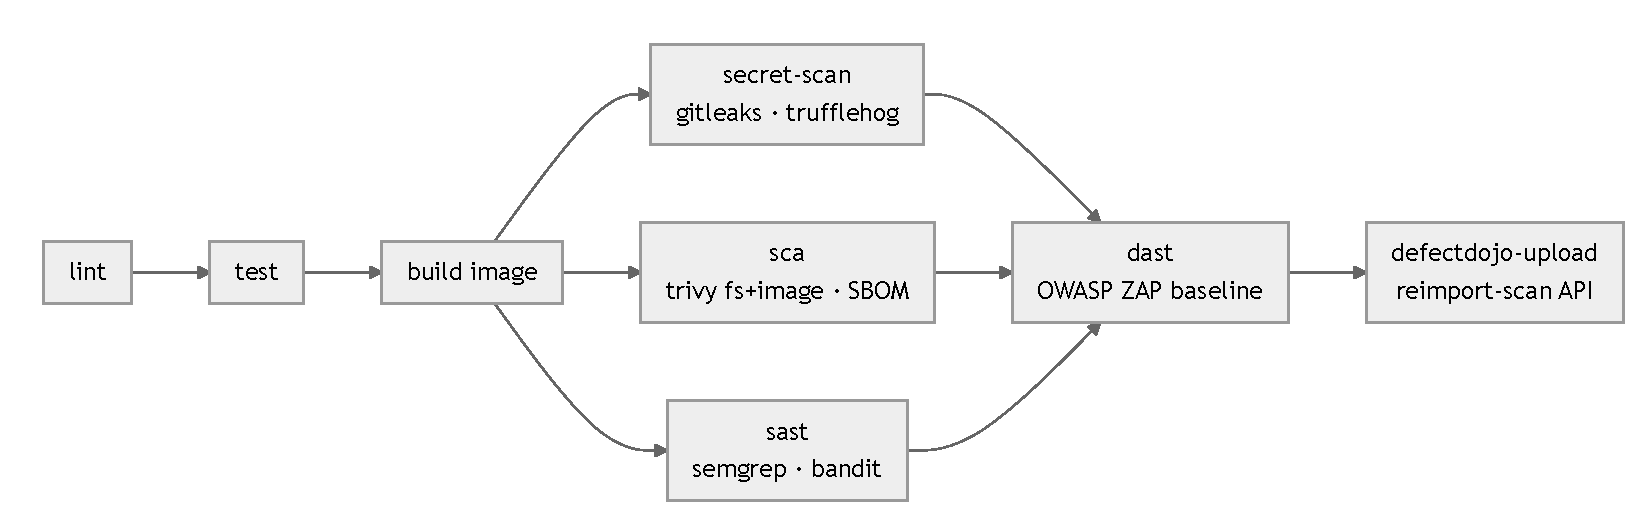
\includegraphics[width=\linewidth]{images/pipeline.pdf}
\end{center}
Los jobs \texttt{lint} y \texttt{test} permanecen en \texttt{ci.yml}. Los escaneos ligeros (secret-scan, SAST,
SCA de filesystem) corren en cada push/PR; los pesados (ZAP DAST, Trivy \emph{image}) se limitan a \texttt{main}
y a un \emph{schedule} semanal. Todos los jobs son no bloqueantes (\emph{allow\_failure-first}).

\subsection{Evidencia: ejecución real en GitHub Actions}
\begin{center}
  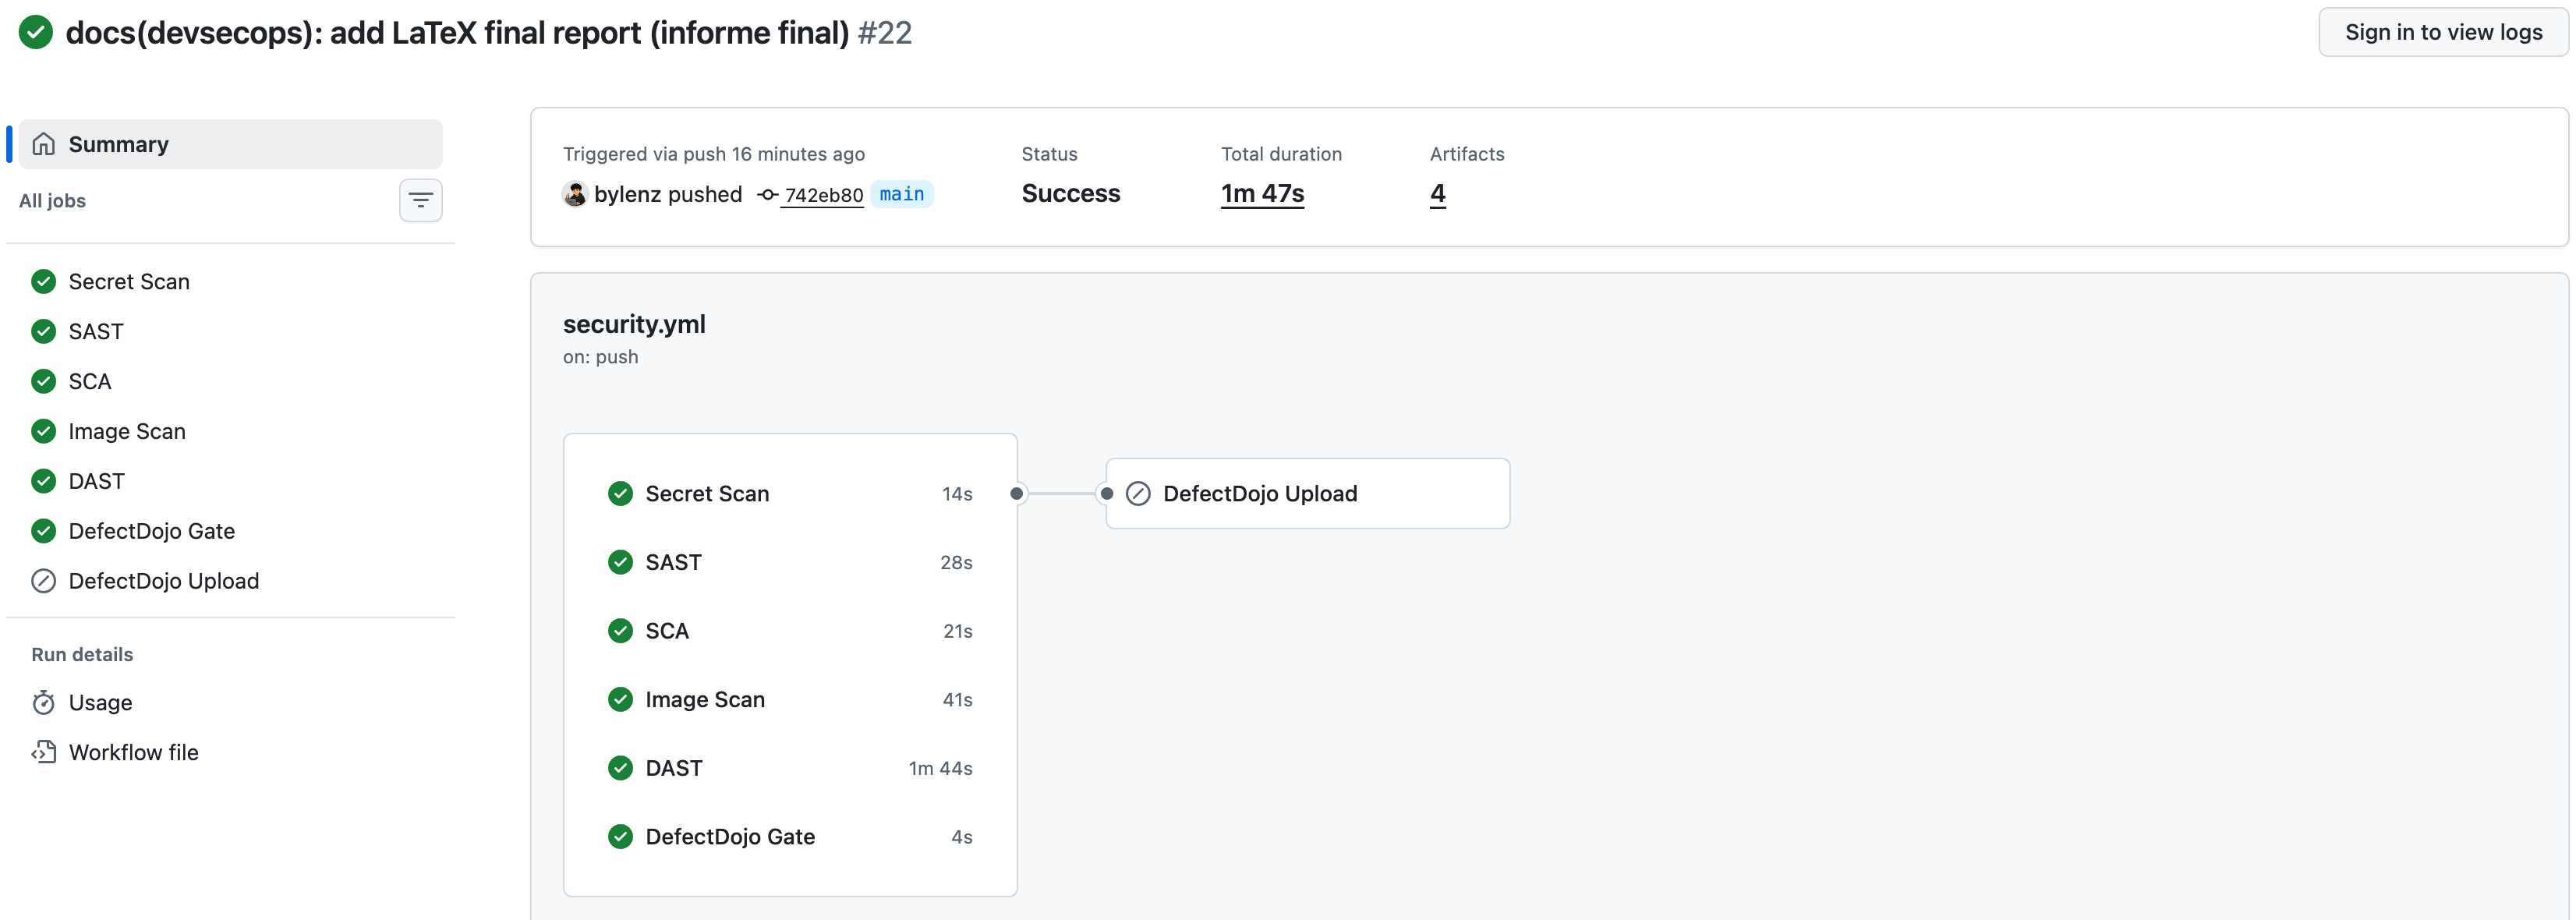
\includegraphics[width=\linewidth]{images/pipeline-github.png}
  \captionof{figure}{Run del workflow \texttt{security.yml} en GitHub Actions (push a \texttt{main}): estado \emph{Success} en 1m\,47s, con el grafo de jobs Secret Scan, SAST, SCA, Image Scan, DAST y DefectDojo Gate $\rightarrow$ DefectDojo Upload (este último \emph{skipped}: sin secreto configurado, comportamiento \emph{evidence-on-demand}).}
\end{center}
\begin{center}
  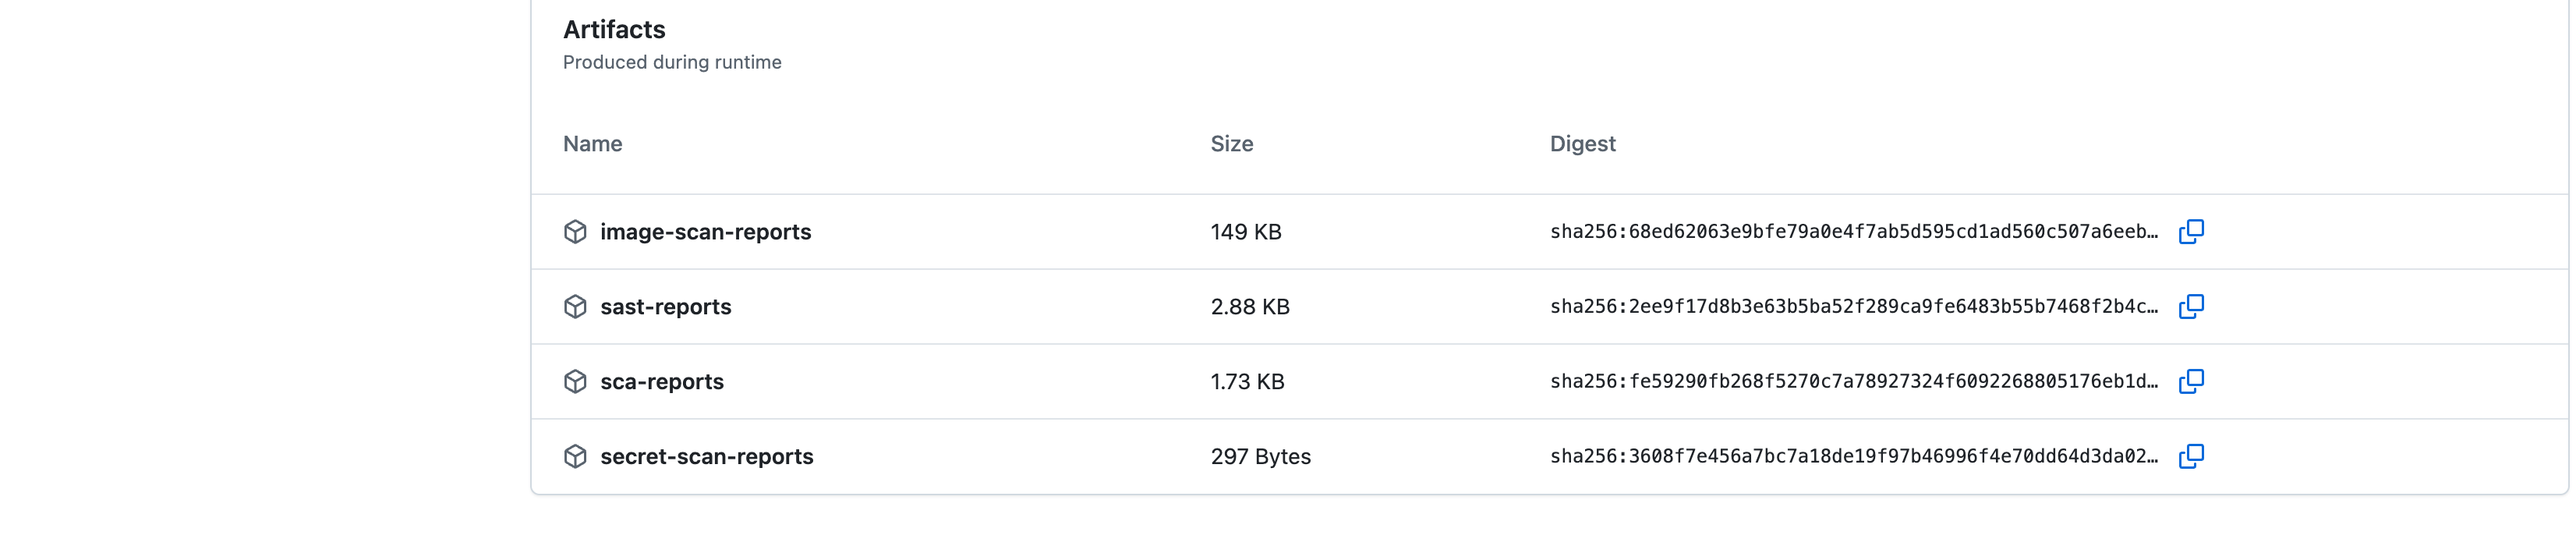
\includegraphics[width=0.92\linewidth]{images/pipeline-artifacts.png}
  \captionof{figure}{Artefactos generados por el pipeline: reportes de los escáneres (\texttt{image-scan-reports}, \texttt{sast-reports}, \texttt{sca-reports}, \texttt{secret-scan-reports}).}
\end{center}

\subsection{Script de configuración (\texttt{.github/workflows/security.yml})}
Extracto representativo (archivo completo en el repositorio):

\begin{lstlisting}[style=yaml]
name: security
on:
  push: { branches: [main, develop] }
  pull_request: { branches: [main, develop] }
  schedule: [{ cron: "0 6 * * 1" }]
  workflow_dispatch:
permissions: { contents: read }

jobs:
  secret-scan:
    runs-on: ubuntu-latest
    if: ${{ github.event_name != 'schedule' }}
    continue-on-error: true
    steps:
      - uses: actions/checkout@v4
        with: { fetch-depth: 0 }
      - run: mkdir -p reports
      - name: Gitleaks
        run: docker run --rm -v "$PWD:/repo" zricethezav/gitleaks:v8.27.2 detect
             --source /repo --report-format json
             --report-path /repo/reports/gitleaks-report.json --exit-code 0 || true
      - name: TruffleHog
        run: docker run --rm -v "$PWD:/repo" ghcr.io/trufflesecurity/trufflehog:3.90.8
             filesystem /repo --results=verified,unknown --json
             > reports/trufflehog-report.json || true
      - uses: actions/upload-artifact@v4
        with: { name: secret-scan-reports, path: reports/ }

  sast:
    runs-on: ubuntu-latest
    if: ${{ github.event_name != 'schedule' }}
    continue-on-error: true
    steps:
      - uses: actions/checkout@v4
      - run: mkdir -p reports
      - name: Semgrep
        run: pipx run semgrep scan --config p/ci --config p/security-audit
             --config p/python --json --output reports/semgrep-report.json
             backend/src/finsight || true
      - name: Bandit
        run: pipx run bandit -r backend/src/finsight -f json
             -o reports/bandit-report.json || true
      - uses: actions/upload-artifact@v4
        with: { name: sast-reports, path: reports/ }

  sca:
    runs-on: ubuntu-latest
    continue-on-error: true
    steps:
      - uses: actions/checkout@v4
      - name: Trivy filesystem (deps)
        uses: aquasecurity/trivy-action@v0.36.0
        with: { scan-type: fs, scan-ref: ., format: json,
                output: reports/trivy-fs-report.json, severity: HIGH,CRITICAL }
      - name: Trivy SBOM (CycloneDX)
        uses: aquasecurity/trivy-action@v0.36.0
        with: { scan-type: fs, scan-ref: ., format: cyclonedx, output: reports/sbom.json }
      - uses: actions/upload-artifact@v4
        with: { name: sca-reports, path: reports/ }

  dast:
    runs-on: ubuntu-latest
    if: ${{ github.event_name == 'schedule' || github.event_name == 'workflow_dispatch'
            || (github.event_name == 'push' && github.ref == 'refs/heads/main') }}
    continue-on-error: true
    steps:
      - uses: actions/checkout@v4
      - run: docker compose up -d --build web db
      - name: Wait for /health
        run: for i in $(seq 1 30); do curl -sf http://localhost:8000/health && break; sleep 5; done
      - name: OWASP ZAP baseline
        uses: zaproxy/action-baseline@v0.12.0
        with: { target: 'http://localhost:8000', fail_action: false }

  defectdojo-gate:
    runs-on: ubuntu-latest
    steps:
      - id: check
        env: { DEFECTDOJO_URL: '${{ secrets.DEFECTDOJO_URL }}' }
        run: echo "enabled=$([ -n "$DEFECTDOJO_URL" ] && echo true || echo false)" >> "$GITHUB_OUTPUT"
    outputs: { enabled: '${{ steps.check.outputs.enabled }}' }

  defectdojo-upload:
    runs-on: ubuntu-latest
    needs: [defectdojo-gate, secret-scan, sast, sca, dast]
    if: ${{ always() && needs.defectdojo-gate.outputs.enabled == 'true' }}
    continue-on-error: true
    steps:
      - uses: actions/checkout@v4
      - uses: actions/download-artifact@v4
      - name: Upload reports to DefectDojo (reimport-scan)
        env:
          DEFECTDOJO_URL: ${{ secrets.DEFECTDOJO_URL }}
          DEFECTDOJO_TOKEN: ${{ secrets.DEFECTDOJO_TOKEN }}
          DEFECTDOJO_PRODUCT_ID: ${{ secrets.DEFECTDOJO_PRODUCT_ID }}
        run: |
          bash scripts/upload_to_defectdojo.sh "Gitleaks Scan"       reports/gitleaks-report.json
          bash scripts/upload_to_defectdojo.sh "Semgrep JSON Report" reports/semgrep-report.json
          bash scripts/upload_to_defectdojo.sh "Bandit Scan"         reports/bandit-report.json
          bash scripts/upload_to_defectdojo.sh "Trivy Scan FS"       reports/trivy-fs-report.json "Trivy Scan"
\end{lstlisting}

\noindent\emph{Nota de implementación:} \texttt{secrets} no está disponible en el \texttt{if:} a nivel de job
en GitHub Actions; por eso el job \texttt{defectdojo-gate} expone la presencia del secreto como un
\emph{output} booleano que \texttt{defectdojo-upload} consume.

% ---------------- j. Lecciones aprendidas ----------------
\section{Lecciones aprendidas (justificación del uso de DevOps)}
\begin{enumerate}[label=\textbf{\arabic*.}]
  \item \textbf{Problema de negocio:} FinSight maneja datos financieros personales (PII). Una filtración o un
        acceso indebido entre hogares destruye la propuesta \emph{privacy-first} y la confianza del usuario.
  \item \textbf{Limitaciones antes:} la seguridad dependía de revisión manual y disciplina individual; las
        vulnerabilidades eran invisibles hasta producción y no había forma de medir la postura de seguridad.
  \item \textbf{Qué cambió con DevOps:} la seguridad se volvió \emph{código} y parte del pipeline
        (\emph{shift-left}). Cada push ejecuta SAST, DAST, SCA y secret scanning, y los hallazgos se
        centralizan automáticamente en DefectDojo.
  \item \textbf{Ventajas concretas:} detección temprana y automática de CVEs y secretos; trazabilidad y
        priorización de hallazgos; doble barrera contra secretos; y un proceso repetible que no depende de
        que alguien recuerde revisar. Además, 4 amenazas STRIDE fueron mitigadas en el código con TDD estricto
        (cobertura backend $\ge 90\%$).
\end{enumerate}

% ---------------- k. Recomendaciones ----------------
\section{Recomendaciones para implementar DevOps en otros proyectos}
\begin{enumerate}[label=\textbf{\arabic*.}]
  \item Empezar por \emph{shift-left}: integrar secret scanning y SCA primero --- baratos, rápidos y de alto impacto.
  \item Doble barrera \emph{pre-commit} + CI: detener problemas antes del push y revalidarlos en el pipeline.
  \item Centralizar hallazgos (DefectDojo) para no perderlos en logs de CI y poder priorizar por severidad.
  \item Modelar amenazas temprano (STRIDE): dirige qué controles importan según el contexto del negocio.
  \item \texttt{allow\_failure} al inicio y \emph{gates} después: reportar sin romper el build, y endurecer a
        \emph{fail-on-finding} cuando el equipo madura.
  \item Tratar la seguridad como parte de la \emph{Definition of Done}, no como una fase final aparte.
\end{enumerate}

% ---------------- Entregables ----------------
\section{Entregables y enlaces}
\begin{enumerate}[label=\arabic*.]
  \item \textbf{Repositorio} (código + pipeline): \href{https://github.com/bylenz/finsight}{github.com/bylenz/finsight}
  \item \textbf{Diagrama STRIDE (draw.io):} \texttt{docs/informe-final/stride-finsight.drawio}
  \item \textbf{Plantilla STRIDE (Excel):} \texttt{docs/informe-final/stride-finsight.xlsx}
  \item \textbf{Informe PDF:} este documento.
  \item \textbf{Evidencia:} \texttt{docs/informe-final/evidence/} (capturas DefectDojo).
\end{enumerate}

\end{document}
